\documentclass{transcrypto}
\usepackage[utf8]{inputenc}
\usepackage[english]{babel}
\usepackage[nottoc]{tocbibind}
\usepackage{colortbl}
%\usepackage[table]{xcolor}
\usepackage{dblfloatfix}
\usepackage{xeCJK}
\usepackage[titletoc]{appendix}
\usepackage{appendix}
\setcounter{MaxMatrixCols}{20}
\definecolor{mypink2}{RGB}{215, 44, 118}
\definecolor{green}{rgb}{0.1,0.1,0.1}
\newcommand{\xxxx}{\cellcolor{mypink2}\textcolor{white}{$b'$xxxx}}
\author{Pagidimarri Nagendar\inst{1} \and Ganta Hemanth Sai Kiran\inst{2}}
\institute{Institute ID.: 11840790\\ Branch: Computer Science (CS) \\Email: \email{pagidimarrin@iitbhilai.ac.in} \and
           Institute ID.: 11840500\\ Branch: Computer Science (CS) \\Email: \email{gantak@iitbhilai.ac.in}}
\title[\texttt{iacrtans} class documentation]{\publname}
\subtitle{CS553 Cryptography Term Paper}

\begin{document}
	\maketitle
	\keywords[\publname, ctp, ctp, LaTeX]{PRIDE, Linear layer, Differential Cryptanalysis, Lightweight cipher, Security, Efficiency}
	
	\begin{abstract}
	The PRIDE cipher is a lightweight block cipher which was introduced by Albrecht et al. It appeared for the first time at CRYPTO 2014. It was claimed that PRIDE benefitted from the linear layers in terms of security. In this paper we explore the cipher PRIDE in detail. It is described and implemented using python and different tests are run on it. We will see an 18-round differential attack for which the complexity $ (D,T,M) = (2^{60},2^{66},2^{64}) $ and we look into the linear attack on cipher PRIDE. Then we explore the performance analysis of PRIDE by comparing it with other lightweight block ciphers like SIMON and SPECK. Finally we conclude by making some correction in the complexity of the proposed 18-round differential attack by observing some key captures. We also understand the use of bit-slice implementation in our cipher PRIDE and the role of linear layer in making our cipher win in the security level.
	\end{abstract}
	\newpage
	\tableofcontents{}
	\newpage
	\listoffigures
	%\newpage
	\listoftables
	\newpage
	\section{Introduction}
	In the context of rapid development in every fields of technology, efficiency is a key issue. Lightweight ciphers serve this very purpose of efficiency as they can be implemented in different constrained environments. This does not always means that there is a security and efficiency trade off. Many lightweight ciphers also provide a good amount of security along with efficiency. PRIDE is one of those ciphers along with SIMON, SPECK, PRINCE and LED. PRIDE is introduced in CRYPTO 2014 by Albrecht et al. It is a block cipher with 64-bits blocks which uses SPN structure with 20 round implementation. It was shown that the cipher provides a fine linear layer to enhance the security and it is the reason PRIDE is ranked good in the existing ciphers in terms of security when implemented on 8-bit microcontroller. It is efficient even in terms of efficiency but SPECK and SIMON grabbed the first places in this scenario.
	
	In this paper we implement the cipher in python, test it. Then we analyse the 18-round differential attack on this cipher and also investigate the linear attack. The complexity of differential attack is $ (D,T,M) = (2^{60},2^{66},2^{64}) $ and for linear attack we need 274.9 encryptions with $ 2^{62} $ known plaintexts. We explore the complexity of the same and finally analyze the implementation of PRIDE on 8-bit microcontroller from close. We rank the ciphers based on the results.
	
	We conclude the paper by reporting the error in the 18-round attack in proposing the complexity, and thus observe the capture of the round keys in different rounds to make some necessary changes in it. We also understand the use of bit-slice implementation in our cipher PRIDE and the role of linear layer in making our cipher win in the security level.
	\section{Description}
	Our Given cipher is PRIDE\cite{10.1007/978-3-662-44371-2_4}. Pride, a lightweight Block cipher, was delineated by ``ALBRECHT" et al. The development of ``LINEAR LAYER" is attractively in line, alongside bit-slice implementation for the.
	``8-bit words". PRIDE uses SPN Structure in its internal and provides an adaptive design between security \& coherence.

	%\FloatBarrier
	\begin{table}[H]
		\centering
		\begin{tabular}{|c|c|}
			\hline
			\textbf{SIZE} & \textbf{BITS} \\ \hline
			BLOCK & 64\\ \hline
			KEY & 128\\ \hline
		\end{tabular}
		\caption{Bit-Size information of PRIDE}
	\end{table}
	PRIDE Cipher has 20 rounds.
	
	Master key $K\,=\,k||k'$ of 128-bit is divided into two nibbles $k,\,k'$ of 64-bit each. The first nibble ($ k $) will used for \textbf{Pre-} and \textbf{Post-whitening}. Whereas the second-nibble ($ k' $) will used for \textbf{Key-scheduling} for the generation of rounds.
	\begin{figure}[H]
		\addtolength{\leftskip} {-1cm}
		\addtolength{\rightskip}{-1.5cm}
		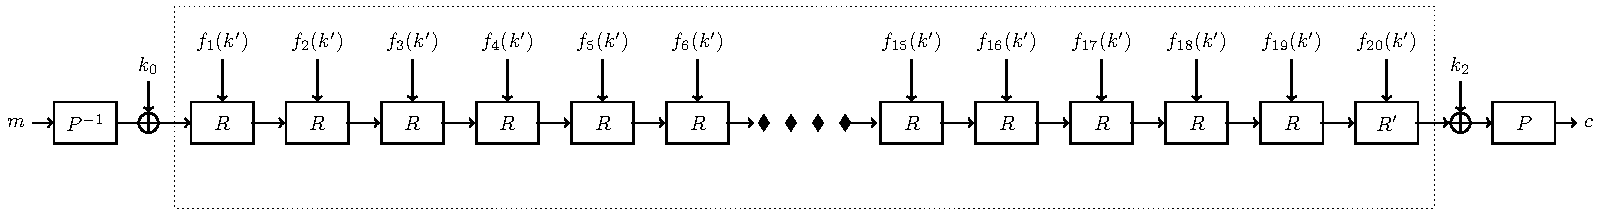
\includegraphics[width=16cm]{structure.pdf}
		\caption{PRIDE - Structure}
		\label{fig1}
	\end{figure}
	\begin{figure}[H]
		\addtolength{\leftskip} {-1cm}
		\addtolength{\rightskip}{-3.5cm}
		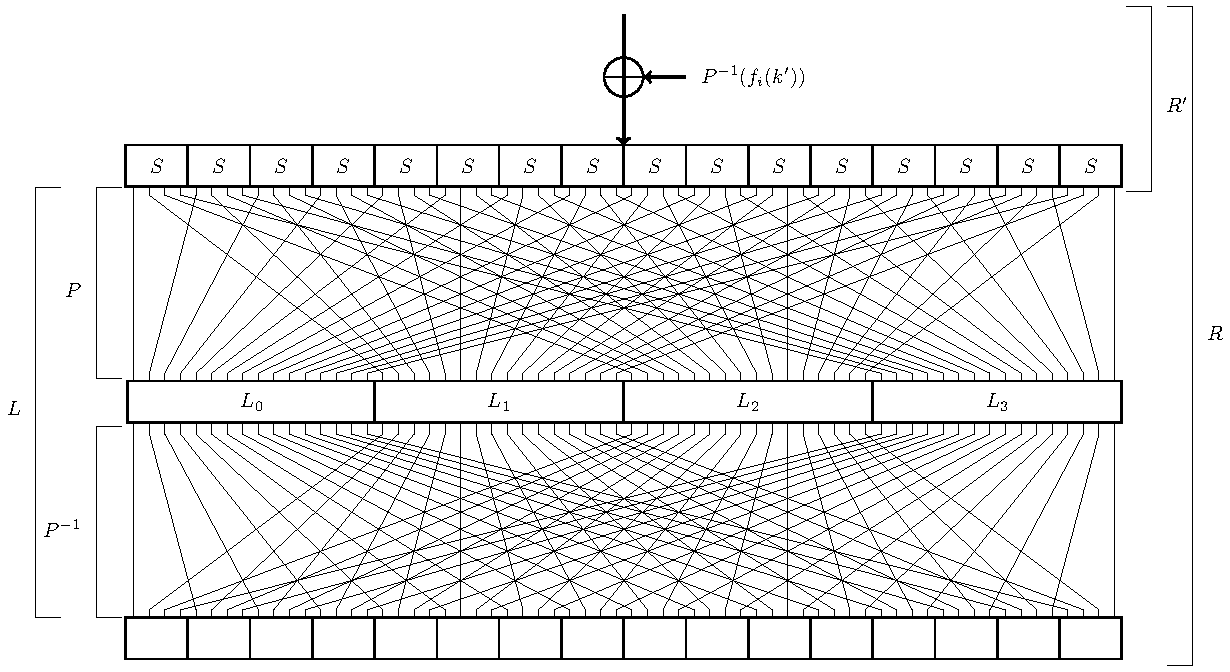
\includegraphics[width=15cm]{pride.pdf}
		\caption{PRIDE - Round function}
		\label{fig2}
	\end{figure}
	\subsection{Round Information}
	Rounds of PRIDE have different operations as given:
	\begin{itemize}
		\item Round-1 to Round-19 : Key addition, Substitution and Linear Layer
		\item Round-20 : Key addition and Substitution
	\end{itemize}
	Different operations of Round functions:
	\begin{enumerate}
		\item \textbf{Key Addition} : Xor-ing the round key and the input of the corresponding round.
		\item \textbf{Substitution} : Output after the key-addition operation is then applied into a 4x4 S-Box (i.e to each nibble of the state).
		\item \textbf{Linear layer} : This consists of 3 different sub-operations
		\begin{enumerate}
			\item Application of bit permutation $P$.
			\item Application of matrix $ L_i $, for $ i = 0,1,2,3 $ to the $ i^{th} $ word (16-bit) of the state.
			\item Application of bit permutation $ P^{-1} $.
		\end{enumerate}
	\end{enumerate}
	$P$, $P^{-1}$ and $L_i$ for $i=0,1,2,3$ are shown in the Appendix \ref{sec}.
	\begin{table}[H]
		\centering
		\begin{tabular}{c|c|c|c|c|c|c|c|c|c|c|c|c|c|c|c|c}
			\hline
			$x$ & 0 & 1 & 2 & 3 & 4 & 5 & 6 & 7 & 8 & 9 & $ a $ & $ b $ & $ c $ & $ d $ & $ e $ & $ f $ \\ \hline
			$S(x)$ & 0 & 4 & 8 & $ f $ & 1 & 5 & $ e $ & 9 & 2 & 7 & $ a $ & $ c $ & $ b $ & $ d $ & 6 & 3 \\ \hline
		\end{tabular}
		\caption{S-box of Cipher PRIDE}
	\end{table}
	\subsection{Key-Schedule}
		After the division from the master key of 128-bit $ (k||k') $, Here from the tuple $ k' $ is divided into 'eight 8-bit' words as shown:
		
		$$ k' = k'_{1}||k'_{2}||k'_{3}||k'_{4}||k'_{5}||k'_{6}||k'_{7}||k'_{8} $$
	
		These 8-bit words are used in key-schedule for generation of the Sub-keys $ f_r(k') $ of different rounds as:
		
		$$ f_r(k') = k'_{1}||g_r^{(1)}(k'_{2})||k'_{3}||g_r^{(2)}(k'_{4})||k'_{5}||g_r^{(3)}(k'_{6})||k'_{7}||g_r^{(4)}(k'_{8})
		 $$
		where $ 1 \le r \le 20 $ and $ g $ function. We can see it in the Table \ref{g} below.
		\begin{table}[H]
			\centering
			\begin{tabular}{|c|l|}
				\hline
				$ g_r^{(1)}(x) $ &  $ (x + 193r) \% $ 256 \\ \hline
				$ g_r^{(2)}(x) $ &  $ (x + 165r) \% $ 256 \\ \hline
				$ g_r^{(3)}(x) $ &  $ (x + 81r) \% $ 256 \\ \hline
				$ g_r^{(4)}(x) $ &  $ (x + 197r) \% $ 256 \\ \hline
			\end{tabular}
			\caption{$g$ function of PRIDE}
			\label{g}
		\end{table}
	\subsection{S-Box Properties}
	\subsubsection{Fixed Points} When we at look at the given S-box, We can clearly observe that in the S-Box, there are 4-fixed points:
	\begin{itemize}
		\item $ S(0) = 0 $
		\item $ S(5) = 5 $
		\item $ S(a) = a $
		\item $ S(d) = d $
	\end{itemize}
	\subsubsection{Component functions of S-Box}
	Let us denote the input nibble of S-Box by $ x = (x_1,x_2,x_3,x_4) $ then the corresponding output nibble is given by $ S(x) = y = (y_1,y_2,y_3,y_4) $.
	We can express $ y $ in terms of $ x $ as follows:
	\begin{align*}
		y_1 &= x_3 \oplus x_1x_2\\ 
		y_2 &= x_4 \oplus x_2x_3\\ 
		y_3 &= x_1 \oplus x_2x_3 \oplus x_3x_4 \oplus x_1x_2x_3 \oplus x_1x_2x_4\\
		y_4 &= x_2 \oplus x_1x_4 \oplus x_2x_3 \oplus x_3x_4 \oplus x_1x_2x_4\\
	\end{align*}
	\textbf{Observations}\\
	$ y_1 $ and $ y_2 $ are depending only on 3 bits out of the 4-bit input which is used in the possible differential transitions of S-Box.
	\subsubsection{Undistrubed bit}
	In the S-box, if we take some particular input difference, we can observe that few bits of output difference remains changed, At that point we can say that those bits are known to be undistrubed.
	
	For example if the input difference is 8 ($b'1000$) then output difference can be \textbf{*0**} where * is a variable bit and 0 remains unchange in any case. Thus it is the undistrubed bit here.
	
	\subsection{Implementation}
	PRIDE cipher is implemented in Python 3, and is tested for different Plaintexts and different keys. We can see the results in Table \ref{e}, \ref{d}.
	\begin{table}[H]
		\centering
		\begin{tabular}{|c|c|c|}
			\hline
			\textbf{Plaintext} ($m$) & \textbf{Key} ($k||k'$) & \textbf{Ciphertext} ($c$) \\ \hline
			8888888888888888 & 4444444444444444   4444444444444444 & 65a0cce60bc0a71a \\ \hline
			4444444444444444 & 8888888888888888   8888888888888888 & 1635c8bf118deac8 \\ \hline
			eeeeeeeeeeeeeeee & abababababababab   abababababababab & e7f8e250641a9c2e \\ \hline
			1010101010101010 & 0101010101010101   0101010101010101 & acb28bb7c57b490d \\ \hline
			abcabcabcabcabca & cbacbacbacbacbac   bacbacbacbacbacb & 51f558e9be909adf \\ \hline
		\end{tabular}
		\caption{Encryption Tests}
		\label{e}
	\end{table}
	\begin{table}[H]
		\centering
		\begin{tabular}{|c|c|c|}
			\hline
			\textbf{Ciphertext} ($m$) & \textbf{Key} ($k||k'$) & \textbf{Plaintext} ($c$) \\ \hline
			65a0cce60bc0a71a & 4444444444444444   4444444444444444  & 8888888888888888\\ \hline
			1635c8bf118deac8 & 8888888888888888   8888888888888888  & 4444444444444444\\ \hline
			e7f8e250641a9c2e & abababababababab   abababababababab  & eeeeeeeeeeeeeeee\\ \hline
			acb28bb7c57b490d & 0101010101010101   0101010101010101  & 1010101010101010\\ \hline
			51f558e9be909adf & cbacbacbacbacbac   bacbacbacbacbacb  & abcabcabcabcabca\\ \hline
		\end{tabular}
		\caption{Decryption Tests}
		\label{d}
	\end{table}
	\section{Notation of PRIDE}
	The notation used throughout the paper from here on:
	\begin{table}[H]
		\centering
		\begin{tabular}{cl}
			
			$ I_r $ & $ r^{th} $ round : \textbf{input}\\ 
			$ X_r $ & $ r^{th} $ round : the state after \textbf{key addition}\\ 
			$ Y_r $ & $ r^{th} $ round : state after \textbf{substitution}\\
			$ Z_r $ & $ r^{th} $ round : state after \textbf{permutation}\\ 
			$ W_r $ & $ r^{th} $ round : state after \textbf{matrix layer}\\ 
			$ O_r $ & $ r^{th} $ round : \textbf{output}\\ 
			$ \Delta X $ & $ X \oplus X_0 $ \\ 
			x & a bit have undetermined value\\ 
			$ X[l_1 , l_2, \dots] $ & state $ X $ with the nibbles $ l_1, l_2, \dots-th $ where $ 1\le l_1 < l_2 < . . . \le 16 $ \\ 
			$ X\{m_1 , m_2, \dots\} $ & state $ X $ with the bits $ m_1, m_2, \dots-th $ where $ 1 \le m_1 < m_2 < \dots \le 64 $,\\
			&enumerated from left to right.\\ 
		\end{tabular}
		\caption{Notation of PRIDE}
		\label{n}
	\end{table}

	\section{Differential Cryptanalysis}
	\begin{table}[H]
		\centering
		\begin{tabular}{c|cccccccccccccccc}
			&0 &  1 &  2 &  3 &  4 &  5 &  6 &  7 &  8 &  9 &  a &  b &  c &  d &  e &  f\\
			\hline 
			0 & 16 &  . &  . &  . &  . &  . &  . &  . &  . &  . &  . &  . &  . &  . &  . &  .\\ 
			1 &  . &  . &  . &  . &  4 &  4 &  4 &  4 &  . &  . &  . &  . &  . &  . &  . &  .\\ 
			2 &  . &  . &  . &  . &  . &  . &  . &  . &  4 &  . &  . &  4 &  2 &  2 &  2 &  2\\ 
			3 &  . &  . &  . &  . &  . &  . &  . &  . &  4 &  . &  . &  4 &  2 &  2 &  2 &  2\\ 
			4 &  . &  4 &  . &  . &  . &  . &  4 &  . &  . &  2 &  2 &  . &  2 &  . &  . &  2\\ 
			5 &  . &  4 &  . &  . &  . &  4 &  . &  . &  . &  2 &  2 &  . &  2 &  . &  . &  2\\ 
			6 &  . &  4 &  . &  . &  4 &  . &  . &  . &  . &  2 &  2 &  . &  . &  2 &  2 &  .\\ 
			7 &  . &  4 &  . &  . &  . &  . &  . &  4 &  . &  2 &  2 &  . &  . &  2 &  2 &  .\\ 
			8 &  . &  . &  4 &  4 &  . &  . &  . &  . &  4 &  . &  4 &  . &  . &  . &  . &  .\\ 
			9 &  . &  . &  . &  . &  2 &  2 &  2 &  2 &  . &  . &  . &  . &  2 &  2 &  2 &  2\\ 
			a &  . &  . &  . &  . &  2 &  2 &  2 &  2 &  4 &  . &  4 &  . &  . &  . &  . &  .\\ 
			b &  . &  . &  4 &  4 &  . &  . &  . &  . &  . &  . &  . &  . &  2 &  2 &  2 &  2\\ 
			c &  . &  . &  2 &  2 &  2 &  2 &  . &  . &  . &  2 &  . &  2 &  2 &  . &  2 &  .\\ 
			d &  . &  . &  2 &  2 &  . &  . &  2 &  2 &  . &  2 &  . &  2 &  . &  2 &  . &  2\\ 
			e &  . &  . &  2 &  2 &  . &  . &  2 &  2 &  . &  2 &  . &  2 &  2 &  . &  2 &  .\\ 
			f &  . &  . &  2 &  2 &  2 &  2 &  . &  . &  . &  2 &  . &  2 &  . &  2 &  . &  2\\  
		\end{tabular}
		\caption{DDT of PRIDE}
	\end{table}
	
	\subsection{18-Round Attack on PRIDE}
	In\cite{cryptoeprint:2014:525} 16 different 2-round iterative characteristics can be found morever we can construct a few 15-round differentials from them. Thus 18-rounds of PRIDE are attacked with \textbf{$ (D,T,M) = (2^{60},2^{66},2^{64}) $}.
	\subsubsection{Differential characteristic of 18-Round attack}
	For the chosen S-Box, input difference $ b'1000 $ leads to the output difference $b'1000$  with a probability of $ \frac{4}{16} = \frac{1}{4} $. Authors of the attack have found 2-round iterative differential characteristic alongside the probability of $ \frac{1}{2^{8}} $ as per the Table \ref{2-round}.
	\begin{center}
	\begin{table}[h]
		\addtolength{\leftskip} {-3cm}
		\addtolength{\rightskip}{-2cm}
		\resizebox{1.45\textwidth}{!}{\begin{tabular*}{1.750\textwidth}{|c|c|c|c|c|c|c|c|c|c|c|c|c|c|c|c|c|}
			\hline
			$ \Delta I _{r} $ & $b'0000$ & $b'1000$ & $b'0000$ & $b'0000$ & $b'0000$ & $b'0000$ & $b'0000$ & $b'0000$ & $b'0000$ & $b'0000$ & $b'0000$ & $b'0000$ & $b'0000$ & $b40000$ & $b'0000$ & $b'0000$ \\ \hline 
			$ \Delta X _{r} $ & $b'0000$ & $b'1000$ & $b'0000$ & $b'0000$ & $b'0000$ & $b'0000$ & $b'0000$ & $b'0000$ & $b'0000$ & $b'0000$ & $b'0000$ & $b'0000$ & $b'0000$ & $b'0000$ & $b'0000$ & $b'0000$ \\ \hline 
			$ \Delta Y _{r} $ & $b'0000$ & $b'1000$ & $b'0000$ & $b'0000$ & $b'0000$ & $b'0000$ & $b'0000$ & $b'0000$ & $b'0000$ & $b'0000$ & $b'0000$ & $b'0000$ & $b'0000$ & $b'0000$ & $b'0000$ & $b'0000$ \\ \hline 
			$ \Delta Z _{r} $ & $b'0100$ & $b'0000$ & $b'0000$ & $b'0000$ & $b'0000$ & $b'0000$ & $b'0000$ & $b'0000$ & $b'0000$ & $b'0000$ & $b'0000$ & $b'0000$ & $b'0000$ & $b'0000$ & $b'0000$ & $b'0000$ \\ \hline 
			$ \Delta W _{r} $ & $b'0000$ & $b'0100$ & $b'0100$ & $b'0100$ & $b'0000$ & $b'0000$ & $b'0000$ & $b'0000$ & $b'0000$ & $b'0000$ & $b'0000$ & $b'0000$ & $b'0000$ & $b'0000$ & $b'0000$ & $b'0000$ \\ \hline 
			$ \Delta I _{r+1} $ & $b'0000$ & $b'0000$ & $b'0000$ & $b'0000$ & $b'0000$ & $b'1000$ & $b'0000$ & $b'0000$ & $b'0000$ & $b'1000$ & $b'0000$ & $b'0000$ & $b'0000$ & $b'1000$ & $b'0000$ & $b'0000$ \\ \hline 
			$ \Delta X _{r+1} $ & $b'0000$ & $b'0000$ & $b'0000$ & $b'0000$ & $b'0000$ & $b'1000$ & $b'0000$ & $b'0000$ & $b'0000$ & $b'1000$ & $b'0000$ & $b'0000$ & $b'0000$ & $b'1000$ & $b'0000$ & $b'0000$ \\ \hline 
			$ \Delta Y _{r+1} $ & $b'0000$ & $b'0000$ & $b'0000$ & $b'0000$ & $b'0000$ & $b'1000$ & $b'0000$ & $b'0000$ & $b'0000$ & $b'1000$ & $b'0000$ & $b'0000$ & $b'0000$ & $b'1000$ & $b'0000$ & $b'0000$ \\ \hline 
			$ \Delta Z _{r+1} $ & $b'0000$ & $b'0100$ & $b'0100$ & $b'0100$ & $b'0000$ & $b'0000$ & $b'0000$ & $b'0000$ & $b'0000$ & $b'0000$ & $b'0000$ & $b'0000$ & $b'0000$ & $b'0000$ & $b'0000$ & $b'0000$ \\ \hline 
			$ \Delta W _{r+1} $ & $b'0100$ & $b'0000$ & $b'0000$ & $b'0000$ & $b'0000$ & $b'0000$ & $b'0000$ & $b'0000$ & $b'0000$ & $b'0000$ & $b'0000$ & $b'0000$ & $b'0000$ & $b'0000$ & $b'0000$ & $b'0000$ \\ \hline 
			$ \Delta I _{r+2} $ & $b'0000$ & $b'1000$ & $b'0000$ & $b'0000$ & $b'0000$ & $b'0000$ & $b'0000$ & $b'0000$ & $b'0000$ & $b'0000$ & $b'0000$ & $b'0000$ & $b'0000$ & $b'0000$ & $b'0000$ & $b'0000$ \\ \hline
		\end{tabular*}}
	\caption{2-Round Differential Characteristic of PRIDE}
	\label{2-round}
	\end{table}
	\end{center}
	\newpage
	As per the Table \ref{162-round} it is found that there are sixteen 2-Round iterative differential characteristics. 
	\begin{table}[H]
		\centering
		\begin{tabular}{ccccc}
			(8000000000000000) & $\overset{1r}{\rightarrow}$ & (0000800080008000) & $\overset{1r}{\rightarrow}$ & (8000000000000000) \\
			
			(0800000000000000) & $\overset{1r}{\rightarrow}$ & (0000080008000800) & $\overset{1r}{\rightarrow}$ & (0800000000000000) \\
			
			(0080000000000000) & $\overset{1r}{\rightarrow}$ & (0000800000800080) & $\overset{1r}{\rightarrow}$ & (0080000000000000) \\
			
			& & \dots & & \\
			
			(0000000000000800) & $\overset{1r}{\rightarrow}$ & (0800080008000000) & $\overset{1r}{\rightarrow}$ & (0000000000000800) \\
			
			(0000000000000080) & $\overset{1r}{\rightarrow}$ & (0080008000800000) & $\overset{1r}{\rightarrow}$ & (8000000000000080) \\
			
			(0000000000000008) & $\overset{1r}{\rightarrow}$ & (0008000800080000) & $\overset{1r}{\rightarrow}$ & (0000000000000008) \\
		\end{tabular}
	\caption{sixteen 2-Round differential characteristics}
	\label{162-round}
	\end{table}
	15-round differential characteristic = 7 2-round differential at the top + 1 1-round differential at the bottom
	
	Probability of 15-round differential characteristic = $ \frac{1}{2^{58}} $
	\begin{center}
		\begin{table}[h]
			\addtolength{\leftskip} {-3cm}
			\addtolength{\rightskip}{-2cm}
			\resizebox{1.45\textwidth}{!}{\begin{tabular*}{1.750\textwidth}{|c|c|c|c|c|c|c|c|c|c|c|c|c|c|c|c|c|}
				\hline
				$ \Delta I_{r} $ & $b'0000$ & $b'1000$ & $b'0000$ & $b'0000$ & $b'0000$ & $b'0000$ & $b'0000$ & $b'0000$ & $b'0000$ & $b'0000$ & $b'0000$ & $b'0000$ & $b'0000$ & $b'0000$ & $b'0000$ & $b'0000$  \\ \hline
				$ \Delta X_{r+15} $ & $b'0000$ & $b'0000$ & $b'0000$ & $b'0000$ & $b'0000$ & $b'1000$ & $b'0000$ & $b'0000$ & $b'0000$ & $b'1000$ & $b'0000$ & $b'0000$ & $b'0000$ & $b'1000$ & $b'0000$ & $b'0000$  \\
				\hline
			\end{tabular*}}
			\caption{15-Round Differential Characteristic for PRIDE}
			\label{15-round}
		\end{table}
	\end{center}
	Similarly, we can build the 18-Round attack as:\\
	18-round differential attack = 1 1-round differential at the top + 15-round differential in the middle + 2 1-round differential at the bottom
	\begin{center}
		\begin{table}[h]
			\addtolength{\leftskip} {-3cm}
			\addtolength{\rightskip}{-2cm}
			\resizebox{1.45\textwidth}{!}{\begin{tabular*}{1.765\textwidth}{@{\extracolsep{\fill}}|c|c|c|c|c|c|c|c|c|c|c|c|c|c|c|c|c|}
				\hline
				$ \Delta I_1 $ & $b'0000$ & $b'0000$ & $b'0000$ & $b'0000$ & $b'0000$ & $b'$xxxx & $b'0000$ & $b'0000$ & $b'0000$ & $b'$xxxx & $b'0000$ & $b'0000$ & $b'0000$ & $b'$xxxx & $b'0000$ & $b'0000$  \\ \hline 
				$ \Delta X_1 $ & $b'0000$ & $b'0000$ & $b'0000$ & $b'0000$ & $b'0000$ & $b'$xxxx & $b'0000$ & $b'0000$ & $b'0000$ & $b'$xxxx & $b'0000$ & $b'0000$ & $b'0000$ & $b'$xxxx & $b'0000$ & $b'0000$  \\ \hline 
				$ \Delta Y_1 $ & $b'0000$ & $b'0000$ & $b'0000$ & $b'0000$ & $b'0000$ & $b'1000$ & $b'0000$ & $b'0000$ & $b'0000$ & $b'1000$ & $b'0000$ & $b'0000$ & $b'0000$ & $b'1000$ & $b'0000$ & $b'0000$  \\ \hline 
				$ \Delta Z_1 $ & $b'0000$ & $b'0100$ & $b'0100$ & $b'0100$ & $b'0000$ & $b'0000$ & $b'0000$ & $b'0000$ & $b'0000$ & $b'0000$ & $b'0000$ & $b'0000$ & $b'0000$ & $b'0000$ & $b'0000$ & $b'0000$  \\ \hline 
				$ \Delta W_1 $ & $b'0100$ & $b'0000$ & $b'0000$ & $b'0000$ & $b'0000$ & $b'0000$ & $b'0000$ & $b'0000$ & $b'0000$ & $b'0000$ & $b'0000$ & $b'0000$ & $b'0000$ & $b'0000$ & $b'0000$ & $b'0000$  \\ \hline 
				$ \Delta I_2 $ & $b'0000$ & $b'1000$ & $b'0000$ & $b'0000$ & $b'0000$ & $b'0000$ & $b'0000$ & $b'0000$ & $b'0000$ & $b'0000$ & $b'0000$ & $b'0000$ & $b'0000$ & $b'0000$ & $b'0000$ & $b'0000$  \\ \hline 
				$ \Delta X_{17} $ & $b'0000$ & $b'0000$ & $b'0000$ & $b'0000$ & $b'0000$ & $b'1000$ & $b'0000$ & $b'0000$ & $b'0000$ & $b'1000$ & $b'0000$ & $b'0000$ & $b'0000$ & $b'1000$ & $b'0000$ & $b'0000$  \\ \hline 
				$ \Delta Y_{17} $ & $b'0000$ & $b'0000$ & $b'0000$ & $b'0000$ & $b'0000$ & $b'$xxxx & $b'0000$ & $b'0000$ & $b'0000$ & $b'$xxxx & $b'0000$ & $b'0000$ & $b'0000$ & $b'$xxxx & $b'0000$ & $b'0000$  \\ \hline 
				$ \Delta Z_{17} $ & $b'0000$ & $b'$0x00 & $b'$0x00 & $b'$0x00 & $b'0000$ & $b'$0x00 & $b'$0x00 & $b'$0x00 & $b'0000$ & $b'$0x00 & $b'$0x00 & $b'$0x00 & $b'0000$ & $b'$0x00 & $b'$0x00 & $b'$0x00  \\ \hline 
				$ \Delta W_{17} $ & $b'$0x00 & $b'$0x00 & $b'$0x00 & $b'$0x00 & $b'$0xxx & $b'$xxx0 & $b'$0xx0 & $b'$0xx0 & $b'$xxx0 & $b'$0xxx & $b'$0xx0 & $b'$0xx0 & $b'$0x00 & $b'$0x00 & $b'$0x00 & $b'$0x00  \\ \hline 
				$ \Delta I_{18} $ & $b'$0xxx & $b'$x0xx & $b'$0xx0 & $b'0000$ & $b'$0x00 & $b'$xx0x & $b'$0xx0 & $b'0000$ & $b'0000$ & $b'$xxxx & $b'$0xxx & $b'0000$ & $b'0000$ & $b'$xxxx & $b'$0x00 & $b'0000$  \\ \hline 
				$ \Delta X_{18} $ & $b'$0xxx & $b'$x0xx & $b'$0xx0 & $b'0000$ & $b'$0x00 & $b'$xx0x & $b'$0xx0 & $b'0000$ & $b'0000$ & $b'$xxxx & $b'$0xxx & $b'0000$ & $b'0000$ & $b'$xxxx & $b'$0x00 & $b'0000$  \\ \hline 
				$ \Delta Y_{18} $ & $b'$xxxx & $b'$xxxx & $b'$xxxx & $b'0000$ & $b'$xxxx & $b'$xxxx & $b'$xxxx & $b'0000$ & $b'0000$ & $b'$xxxx & $b'$xxxx & $b'0000$ & $b'0000$ & $b'$xxxx & $b'$xxxx & $b'0000$  \\ \hline 
				$ \Delta O_{18} $ & $b'$xxxx & $b'$xxxx & $b'$xxxx & $b'0000$ & $b'$xxxx & $b'$xxxx & $b'$xxxx & $b'0000$ & $b'0000$ & $b'$xxxx & $b'$xxxx & $b'0000$ & $b'0000$ & $b'$xxxx & $b'$xxxx & $b'0000$ \\
				\hline
			\end{tabular*}}
			\caption{18-round differential attack for PRIDE}
			\label{18-round}
		\end{table}
	\end{center}
	\subsubsection{Data Collection}
	In this juncture, we choose $ 2^{n} $ structures, where in each of the plaintext nibbles 1,2,3,4,5,7,8,9,\\11,12,13,14,15,16 are fixed and 6,10,14 are variable. So for these nibbles we have $ 2^{23} $ plaintext and ciphertext pairs. From the Table \ref{18-round}, for these selected plaintexts, At the end of 18-rounds ciphertext difference must satisfy the difference of nibbles (4,8,9,12,13,16) should be 0. As it has a possibility of $ 2^{4} $ of each nibble, thus the probability is $ \frac{1}{{2^{4}}^{6}} = 2^{-24} $. Thus the total no. of pairs = $ 2^{-1} $.
	\subsubsection{Key-Recovery}
	Here, structures $ 2^{n} $ were chosen. The 64 bits of the key are guessed.
	\begin{center}
	\begin{table}[h]
		\addtolength{\leftskip} {-3cm}
		\addtolength{\rightskip}{-2cm}
		\resizebox{1.45\textwidth}{!}{\begin{tabular*}{1.765\textwidth}{|c|c|c|c|c|c|c|c|c|c|c|c|c|c|c|c|c|}
			\hline 
			$ \Delta I_{1} $ & $b'0000$ & $b'0000$ & $b'0000$ & $b'0000$ & $b'0000$ & $b'$xxxx & $b'0000$ & $b'0000$ & $b'0000$ & $b'$xxxx & $b'0000$ & $b'0000$ & $b'0000$ & $b'$xxxx & $b'0000$ & $b'0000$    \\ \hline 
			$ \Delta X_{1} $ & $b'0000$ & $b'0000$ & $b'0000$ & $b'0000$ & $b'0000$ & \xxxx & $b'0000$ & $b'0000$ & $b'0000$ & \xxxx & $b'0000$ & $b'0000$ & $b'0000$ & \xxxx & $b'0000$ & $b'0000$    \\ \hline 
			$ \Delta Y_{1} $ & $b'0000$ & $b'0000$ & $b'0000$ & $b'0000$ & $b'0000$ & $b'1000$ & $b'0000$ & $b'0000$ & $b'0000$ & $b'1000$ & $b'0000$ & $b'0000$ & $b'0000$ & $b'1000$ & $b'0000$ & $b'0000$    \\ \hline 
			$ \Delta Z_{1} $ & $b'0000$ & $b'0100$ & $b'0100$ & $b'0100$ & $b'0000$ & $b'0000$ & $b'0000$ & $b'0000$ & $b'0000$ & $b'0000$ & $b'0000$ & $b'0000$ & $b'0000$ & $b'0000$ & $b'0000$ & $b'0000$    \\ \hline 
			$ \Delta W_{1} $ & $b'0100$ & $b'0000$ & $b'0000$ & $b'0000$ & $b'0000$ & $b'0000$ & $b'0000$ & $b'0000$ & $b'0000$ & $b'0000$ & $b'0000$ & $b'0000$ & $b'0000$ & $b'0000$ & $b'0000$ & $b'0000$    \\ \hline 
			$ \Delta I_{2} $ & $b'0000$ & $b'1000$ & $b'0000$ & $b'0000$ & $b'0000$ & $b'0000$ & $b'0000$ & $b'0000$ & $b'0000$ & $b'0000$ & $b'0000$ & $b'0000$ & $b'0000$ & $b'0000$ & $b'0000$ & $b'0000$    \\ \hline 
			\hline
			$ \Delta X_{17} $ & $b'0000$ & $b'0000$ & $b'0000$ & $b'0000$ & $b'0000$ & $b'1000$ & $b'0000$ & $b'0000$ & $b'0000$ & $b'1000$ & $b'0000$ & $b'0000$ & $b'0000$ & $b'1000$ & $b'0000$ & $b'0000$    \\ \hline 
			$ \Delta Y_{17} $ & $b'0000$ & $b'0000$ & $b'0000$ & $b'0000$ & $b'0000$ & \xxxx & $b'0000$ & $b'0000$ & $b'0000$ & \xxxx & $b'0000$ & $b'0000$ & $b'0000$ & \xxxx & $b'0000$ & $b'0000$    \\ \hline 
			$ \Delta Z_{17} $ & $b'0000$ & $b'$0x00 & $b'$0x00 & $b'$0x00 & $b'0000$ & $b'$0x00 & $b'$0x00 & $b'$0x00 & $b'0000$ & $b'$0x00 & $b'$0x00 & $b'$0x00 & $b'0000$ & $b'$0x00 & $b'$0x00 & $b'$0x00    \\ \hline 
			$ \Delta W_{17} $ & $b'$0x00 & $b'$0x00 & $b'$0x00 & $b'$0x00 & $b'$0xxx & $b'$xxx0 & $b'$0xx0 & $b'$0xx0 & $b'$xxx0 & $b'$0xxx & $b'$0xx0 & $b'$0xx0 & $b'$0x00 & $b'$0x00 & $b'$0x00 & $b'$0x00    \\ \hline 
			$ \Delta I_{18} $ & $b'$0xxx & $b'$x0xx & $b'$0xx0 & $b'0000$ & $b'$0x00 & $b'$xx0x & $b'$0xx0 & $b'0000$ & $b'0000$ & $b'$xxxx & $b'$0xxx & $b'0000$ & $b'0000$ & $b'$xxxx & $b'$0x00 & $b'0000$    \\ \hline 
			$ \Delta X_{18} $ & $b'$0xxx & $b'$x0xx & $b'$0xx0 & $b'0000$ & $b'$0x00 & $b'$xx0x & $b'$0xx0 & $b'0000$ & $b'0000$ & $b'$xxxx & $b'$0xxx & $b'0000$ & $b'0000$ & $b'$xxxx & $b'$0x00 & $b'0000$    \\ \hline 
			$ \Delta Y_{18} $ & \xxxx & \xxxx & \xxxx & $b'0000$ & \xxxx & \xxxx & \xxxx & $b'0000$ & $b'0000$ & \xxxx & \xxxx & $b'0000$ & $b'0000$ & \xxxx & \xxxx & $b'0000$    \\ \hline 
			$ \Delta O_{18} $ & $b'$xxxx & $b'$xxxx & $b'$xxxx & $b'0000$ & $b'$xxxx & $b'$xxxx & $b'$xxxx & $b'0000$ & $b'0000$ & $b'$xxxx & $b'$xxxx & $b'0000$ & $b'0000$ & $b'$xxxx & $b'$xxxx & $b'0000$    \\ \hline
		\end{tabular*}}
		\caption{Key bit guess in 18 - Rounds \textbf{Differential attack} of PRIDE}
		\label{guessed}
	\end{table}
	From Table \ref{guessed}, guesses key nibbles (highlighted) are:
	\begin{itemize}
		\item X[6],X[10],X[14] - Round-1 
		\item Y[6],Y[10],Y[14] - Round-17
		\item Y[1],Y[2],Y[3],Y[5],Y[6],Y[7],Y[10],Y[11],Y[14],Y[15] - Round-18
	\end{itemize}
	\end{center}
	\textbf{Step-1}: \\
	- Encryption of nibble $ X_1[6] $\\
	- Distinguishing the pairs whose output difference $ \Delta Y_1[6] = b'1000 $\\
	- key bits of $ X_1[6] $ are guessed\\
	- No. of pairs remaining = $ 2^{-5} $ \\ \\
	\textbf{Step-2}: \\
	- Encryption of nibble $ X_1[10] $\\
	- Distinguishing the pairs whose output difference $ \Delta Y_1[10] = b'1000 $\\
	- key bits of $ X_1[10] $ are guessed\\
	- No. of pairs remaining = $ 2^{-9} $\\ \\
	\textbf{Step-3}: \\
	- Encryption of nibble $ X_1[14] $\\
	- Distinguishing the pairs whose output difference $ \Delta Y_1[14] = b'1000 $\\
	- key bits of $ X_1[14] $ are guessed\\
	- No. of pairs remaining = $ 2^{-13} $\\ \\
	\textbf{Step-4}:\\
	- Decryption of $ Y_{18}[15],Y_{18}[14],Y_{18}[11],Y_{18}[10],Y_{18}[7],Y_{18}[6],Y_{18}[5],Y_{18}[3],Y_{18}[2],Y_{18}[1] $\\
	- Distinguish the pairs by their factors of $ 2^{-3},2^{-3},2^{-1},2^{-2},2^{-3},2^{-1},2^{-2},2^{-0},2^{-1},2^{-0},2^{-3} $ and guessing the corresponding key bits\\
	- No. of pairs remaining = $ 2^{-29} $\\ \\
	\textbf{Step-5}:\\
	- Decryption of remaining pairs without guessing key by distinguishing $ 2^{-12} $ pairs\\
	- No. of pairs remaining = $ 2^{-41} $\\ \\
	\textbf{Step-6}:\\
	- Decryption of nibble $ Y_{17}[6] $\\
	- Distinguishing the pairs whose output difference $ \Delta X_{17}[6] = b'1000 $\\
	- key bits of $ Y_{17}[6] $ are guessed\\
	- No. of pairs remaining = $ 2^{-45} $\\ \\
	\textbf{Step-7}:\\
	- Decryption of nibble $ Y_{17}[10] $\\
	- Distinguishing the pairs whose output difference $ \Delta X_{17}[10] = b'1000 $\\
	- key bits of $ Y_{17}[10] $ are guessed\\
	- No. of pairs remaining = $ 2^{-49} $\\ \\
	\textbf{Step-8}:\\
	- Decryption of nibble $ Y_{17}[14] $\\
	- Distinguishing the pairs whose output difference $ \Delta X_{17}[14] = b'1000 $\\
	- key bits of $ Y_{17}[14] $ are guessed\\
	- No. of pairs remaining = $ 2^{-53} $\\ \\
	\textbf{Step-9}:\\
	- Remaining 64bits are decrypted with exhaustive seaarch\\ \\
	
	Here the value of $n$ was chosen. And it is 48. So $ 2^{48+23} $ pairs are used to guess the keys.
	\subsubsection{Complexity}\label{compl}
	\textbf{Data} : $2^{60}$\\
	\textbf{Time} : $2^{66}$\\
	\begin{table}[h]
		\centering
		\begin{tabular}{|c|c|c|c|}
			\hline
			\textbf{Step} & \textbf{Calculation} & \textbf{No. of encryptions}(Approx.) \\ \hline
			1 & $2 \times 2^{47} \times 2^4 \times 2^{-4} \times 18^{-1}$ & $2^{43}$ \\ \hline
			2 & $2 \times 2^{43} \times 2^4 \times 2^{4} \times 2^{-4} \times 18^{-1}$ & $2^{43}$ \\ \hline
			3 & $2 \times 2^{39} \times 2^8 \times 2^{4} \times 2^{-4} \times 18^{-1}$ & $2^{43}$ \\ \hline
			4 & $2 \times 2^{19} \times 2^{48} \times 2^4 \times 2^{-4} \times 18^{-1}$ & $2^{62}$ \\ \hline
			5 & $2 \times 2^{19} \times 2^{52} \times 2^{-2} \times 18^{-1}$ & \textbf{$2^{66}$} \\ \hline
			6 & $2 \times 2^{7} \times 2^{52} \times 2^{4} \times 2^{-4} \times 18^{-1}$ & $2^{55}$ \\ \hline
			7 & $2 \times 2^{3} \times 2^{56} \times 2^{4} \times 2^{-4} \times 18^{-1}$ & $2^{55}$ \\ \hline
			8 & $2 \times 2^{-1} \times 2^{60} \times 2^{4} \times 2^{-4} \times 18^{-1}$ & $2^{55}$ \\ \hline
		\end{tabular}
	\caption{Time complexity of the 18-round attack}
	\end{table}
	\textbf{Memory} : $2^{64}$
	
	\section{Linear Cryptanalysis}
	\begin{table}[H]
		\centering
		\begin{tabular}{c|cccccccccccccccc}
			&0 &  1 &  2 &  3 &  4 &  5 &  6 &  7 &  8 &  9 &  a &  b &  c &  d &  e &  f\\
			\hline 
			0 &   +8 &    . &    . &    . &    . &    . &    . &    . &    . &    . &    . &    . &    . &    . &    . &    .\\
			1 &    . &   +4 &   -2 &   -2 &   +4 &    . &   +2 &   +2 &    . &    . &   +2 &   -2 &    . &    . &   +2 &   -2\\
			2 &    . &   -2 &   +2 &    . &    . &   +2 &   -2 &    . &   +4 &   +2 &   +2 &    . &    . &   +2 &   +2 &   -4\\
			3 &    . &   -2 &    . &   +2 &   +4 &   -2 &    . &   -2 &    . &   +2 &    . &   -2 &   +4 &   +2 &    . &   +2\\
			4 &    . &   +4 &    . &   +4 &    . &   +4 &    . &   -4 &    . &    . &    . &    . &    . &    . &    . &    .\\
			5 &    . &    . &   +2 &   -2 &   +4 &   +4 &   -2 &   +2 &    . &    . &   -2 &   +2 &    . &    . &   -2 &   +2\\
			6 &    . &   +2 &   -2 &    . &    . &   -2 &   +2 &    . &   +4 &   +2 &   -2 &   +4 &    . &   +2 &   -2 &    .\\
			7 &    . &   +2 &    . &   -2 &   -4 &   +2 &    . &   +2 &    . &   +2 &    . &   -2 &   +4 &   +2 &    . &   +2\\
			8 &    . &    . &   +4 &    . &    . &    . &   +4 &    . &    . &    . &   +4 &    . &    . &    . &   -4 &    .\\
			9 &    . &    . &   +2 &   +2 &    . &    . &   +2 &   +2 &    . &   -4 &   -2 &   +2 &   +4 &    . &   +2 &   -2\\
			a &    . &   +2 &   +2 &    . &    . &   -2 &   -2 &    . &   +4 &   -2 &   +2 &    . &    . &   -2 &   +2 &   +4\\
			b &    . &   -2 &    . &   -2 &    . &   +2 &   +4 &   -2 &    . &   +2 &    . &   +2 &    . &   -2 &   +4 &   +2\\
			c &    . &    . &    . &   +4 &    . &    . &    . &   +4 &    . &   +4 &    . &    . &    . &   -4 &    . &    .\\
			d &    . &    . &   +2 &   +2 &    . &    . &   +2 &   +2 &    . &    . &   -2 &   -2 &   -4 &   +4 &   +2 &   +2\\
			e &    . &   +2 &   +2 &    . &    . &   -2 &   -2 &    . &   -4 &   +2 &   +2 &   +4 &    . &   +2 &   +2 &    .\\
			f &    . &   -2 &   -4 &   +2 &    . &   +2 &    . &   +2 &    . &   -2 &   +4 &   +2 &    . &   +2 &    . &   +2\\
		\end{tabular}
		\caption{LAT of PRIDE}
	\end{table}
	According to \cite{chinese}, 16 different 2-round iterative linear approximations were constructed with a bias of $2^{-5}$ and 8 different 1-round iterative linear approximations were constructed with a bias of $2^{-3}$. With the help of Linear cryptanalysis, and based on some approximations 18- and 19-rounds attacks were presented. This requires the usage of the key schedule properties and the linear characteristics. The requirements are $2^{60}$ known plaintexts for 274.9 encryptions and $2^{62}$ known plaintexts for 274.9 encryptions.
	\section{Implementational Analysis of PRIDE}
	Implementation of block ciphers along with cipher PRIDE on 8-bit microcontrollers \cite{Hatzivasilis2018} revealed a lot of details about of speculations about the performance. The details of the implementation for PRIDE are shown in Table . All fields are self-explanative.
	
	\begin{table}[H]
		\centering
		\begin{tabular}{|c|c|}
			\hline
			\textbf{Field} & \textbf{Value for cipher PRIDE}\\
			\hline
			ROM (byte) & 266\\ \hline
			RAM (byte) & 0\\ \hline
			Latency (cycles/block) & 1514\\ \hline
			Energy (μJ/bit) & 6.0\\ \hline
			Throughput at 4 MHz (Kbps) & 169\\ \hline
			Efficiency (Kbps/KB) & 635.33\\ \hline
		\end{tabular}
	\caption{Cipher PRIDE implementational details}
	\end{table}
	\newpage
	From \cite{Hatzivasilis2018}, we can compare PRIDE with different other lightweight ciphers which outperformed it mostly.
	\begin{itemize}
		\item ROM (byte) for the implementation of PRIDE required 266 bytes while for different variants of SIMON and SPECK it is 170 and 134 (minimum of all for the corresponding) respectively, making them to outperform PRIDE.
		\item RAM (byte) for the cipher PRIDE along with ciphers like SIMON and SPECK is 0, meaning that PRIDE performed on somewhat equal terms with them.
		\item Latency (cycles/block) (how much time occurs between the moment an input byte (or block) is injected, and the corresponding output byte (or block) is obtained) for PRIDE is 1514 cycles/block while for SIMON and SPECK the least is of 901 and 599 respectively making them to win nearly in the race.
		\item Energy (μJ/bit) for PRIDE is 6μJ/bit while for SIMON and SPECK it is 2.3 (for both) at the least, i.e energy spent on a bit is very less upto nearly 50\% compared to PRIDE which effects even other fields.
		\item Throughputs for ciphers like AES, SIMON and SPECK are 256, 323 and 444 respectively whereas for PRIDE it is 169 Kbps which again is making PRIDE bad.
		\item SIMON and SPECK are performing well in terms of efficiency with values equal to 1900.00 Kbps/KB and 3511.19 Kbps/KB while PRIDE has an efficiency of 635.33 Kbps/KB.
	\end{itemize}
	
	Based on the above analysis, we can say that SPECK is dominating in the whole lightweight ciphers with an efficiency of 3511.19Kbps/KB and also in other factors. Coming to SIMON it is getting second place with nearly half the efficiency as of SPECK but is outperforming PRIDE with nearly 2 times efficiency than it. Finally PRIDE is getting 3rd position comparing multiple factors. Thus keeping performance in mind \textbf{SPECK}, \textbf{SIMON} and \textbf{PRIDE} is the order from best to least.
	
	\subsection{Security Comparison}
	Based on FELICS implementations \cite{ciphers:2020} of block ciphers in different scenarios, all we can say about PRIDE is it is secure against any attack (as of now, according to our knowledge) with Security level -1(Security level (Sec.) is the ratio of the number of rounds broken in a single key setting to the total number of rounds) whereas SIMON and SPECK have 0.74 and 0.71 values meaning that they are be breakable. Thus when it comes to security the order is \textbf{PRIDE}, \textbf{SPECK} and \textbf{SIMON}.
	\newpage
	\section{Conclusion}
	In PRIDE we use Bit-sliced implementation mainly for permutation and inverse permutation layers. From S-Box layer, the first S-Boxes bits are sliced and they are permuted as $ (0,1,2,3) \rightarrow (0,16,32,48) $ and the L-layer is applied then. The reverse permutation is implemented vice versa from $ (0,16,32,48) \rightarrow (0,1,2,3) $. All these operations are bit-wise thus we get benefitted from it in many ways like:
	\begin{itemize}
		\item Speed
		\item Parallelization
		\item Constant execution time
	\end{itemize}

	\textbf{Bit-slicing} is useful as it uses single-bit logical operations and thus results in a code which is immune to cache and timing-related side channel attacks.
	
	\textbf{Linear layer} of PRIDE is efficient because it involves block interleaving which reduces the search space. In the search for linear matrices the authors ended up with 36 instructions for the whole linear layer which are $L_0=7,\,L_1=11,\,L_2=7,\,L_3=11,\,{L_0}^{-1}=7,\,{L_1}^{-1}=13,\,{L_2}^{-1}=7,\,{L_3}^{-1}=13$.
	
	\textbf{Correction of the complexity} provided:
	In the described complexity in\\ section \ref{compl} it is said that 40-bits round key is captured in $ 18^{th} $ round key layer, 12-bit key in the $ 17^{th} $ round and 12-bit in $ 1^{st} $ round. This makes the time complexity $2^{64}$ a whole.
	
	This is an error because the differentials in the $ 1^{st} $ and $ 17^{th} $ rounds were unidentified viz $Y_1[10], Y_1[6], Y_1[2]$ and $X_{17}[10], X_{17}[6], X_{17}[2]$. This leads to capturing only 58 bits in place of 64 as said, which make the time complexity $2^{70}$ by correcting $2^{66}$ as it needs exhaustive search.
	
	\section*{Brownie Points}
	\begin{itemize}
		\item The cipher PRIDE given is analyzed for different implementations and it is found out that PRIDE performs best in terms of Security when compared to SPECK and SIMON and other lightweight block ciphers. While SPECK and SIMON outperformed PRIDE in terms of efficiency, the security level of these when ranked will be in the order of:
		\begin{enumerate}
			\item PRIDE
			\item SPECK
			\item SIMON
		\end{enumerate}
		
		\item The proposed complexity of 18-round differential attack $ (D,T,M) = (2^{60},2^{66},2^{64}) $ is again observed and it is found out that there are rounds where round key captures were said to be 64 in place of 58 bits. Re-evaluating the complexity we get $2^{70}$ in place of $(2^{66})$.\\
		So, the complexity now is $ (D,T,M) = (2^{60},2^{70},2^{64}) $
		
		\item Figure \ref{fig1} and \ref{fig2} are drawn using \texttt{$\textbackslash$tikzlibrary} package in latex with cryptographic symbols class.
	\end{itemize}
	
	\newpage
	\bibliographystyle{plain}
	\bibliography{1,2,3,4,5}
	
	
	\begin{appendices}
	\appendix
	\section{Linear layer Operations}
	\label{sec}
	
	\begin{equation*}
	L_0 =  L_0^{-1} = 
	\begin{pmatrix}
	0 & 0 & 0 & 0 & 1 & 0 & 0 & 0 & 1 & 0 & 0 & 0 & 1 & 0 & 0 & 0\\
	0 & 0 & 0 & 0 & 0 & 1 & 0 & 0 & 0 & 1 & 0 & 0 & 0 & 1 & 0 & 0\\
	0 & 0 & 0 & 0 & 0 & 0 & 1 & 0 & 0 & 0 & 1 & 0 & 0 & 0 & 1 & 0\\
	0 & 0 & 0 & 0 & 0 & 0 & 0 & 1 & 0 & 0 & 0 & 1 & 0 & 0 & 0 & 1\\
	1 & 0 & 0 & 0 & 0 & 0 & 0 & 0 & 1 & 0 & 0 & 0 & 1 & 0 & 0 & 0\\
	0 & 1 & 0 & 0 & 0 & 0 & 0 & 0 & 0 & 1 & 0 & 0 & 0 & 1 & 0 & 0\\
	0 & 0 & 1 & 0 & 0 & 0 & 0 & 0 & 0 & 0 & 1 & 0 & 0 & 0 & 1 & 0\\
	0 & 0 & 0 & 1 & 0 & 0 & 0 & 0 & 0 & 0 & 0 & 1 & 0 & 0 & 0 & 1\\
	1 & 0 & 0 & 0 & 1 & 0 & 0 & 0 & 0 & 0 & 0 & 0 & 1 & 0 & 0 & 0\\
	0 & 1 & 0 & 0 & 0 & 1 & 0 & 0 & 0 & 0 & 0 & 0 & 0 & 1 & 0 & 0\\
	0 & 0 & 1 & 0 & 0 & 0 & 1 & 0 & 0 & 0 & 0 & 0 & 0 & 0 & 1 & 0\\   
	0 & 0 & 0 & 1 & 0 & 0 & 0 & 1 & 0 & 0 & 0 & 0 & 0 & 0 & 0 & 1\\
	1 & 0 & 0 & 0 & 1 & 0 & 0 & 0 & 1 & 0 & 0 & 0 & 0 & 0 & 0 & 0\\
	0 & 1 & 0 & 0 & 0 & 1 & 0 & 0 & 0 & 1 & 0 & 0 & 0 & 0 & 0 & 0\\   
	0 & 0 & 1 & 0 & 0 & 0 & 1 & 0 & 0 & 0 & 1 & 0 & 0 & 0 & 0 & 0\\
	0 & 0 & 0 & 1 & 0 & 0 & 0 & 1 & 0 & 0 & 0 & 1 & 0 & 0 & 0 & 0
	\end{pmatrix}
	\end{equation*}
	
	\begin{equation*}
	L_1 = 
	\begin{pmatrix}
	1 & 1 & 0 & 0 & 0 & 0 & 0 & 0 & 0 & 0 & 0 & 1 & 0 & 0 & 0 & 0 \\ 
	0 & 1 & 1 & 0 & 0 & 0 & 0 & 0 & 0 & 0 & 0 & 0 & 1 & 0 & 0 & 0 \\ 
	0 & 0 & 1 & 1 & 0 & 0 & 0 & 0 & 0 & 0 & 0 & 0 & 0 & 1 & 0 & 0  \\ 
	0 & 0 & 0 & 1 & 1 & 0 & 0 & 0 & 0 & 0 & 0 & 0 & 0 & 0 & 1 & 0 \\ 
	0 & 0 & 0 & 0 & 1 & 1 & 0 & 0 & 0 & 0 & 0 & 0 & 0 & 0 & 0 & 1 \\ 
	0 & 0 & 0 & 0 & 0 & 1 & 1 & 0 & 1 & 0 & 0 & 0 & 0 & 0 & 0 & 0   \\ 
	0 & 0 & 0 & 0 & 0 & 0 & 1 & 1 & 0 & 1 & 0 & 0 & 0 & 0 & 0 & 0 \\ 
	1 & 0 & 0 & 0 & 0 & 0 & 0 & 1 & 0 & 0 & 1 & 0 & 0 & 0 & 0 & 0 \\ 
	1 & 0 & 0 & 0 & 0 & 0 & 0 & 0 & 0 & 0 & 0 & 1 & 1 & 0 & 0 & 0 \\ 
	0 & 1 & 0 & 0 & 0 & 0 & 0 & 0 & 0 & 0 & 0 & 0 & 1 & 1 & 0 & 0 \\ 
	0 & 0 & 1 & 0 & 0 & 0 & 0 & 0 & 0 & 0 & 0 & 0 & 0 & 1 & 1 & 0   \\ 
	0 & 0 & 0 & 1 & 0 & 0 & 0 & 0 & 0 & 0 & 0 & 0 & 0 & 0 & 1 & 1 \\ 
	0 & 0 & 0 & 0 & 1 & 0 & 0 & 0 & 1 & 0 & 0 & 0 & 0 & 0 & 0 & 1 \\ 
	0 & 0 & 0 & 0 & 0 & 1 & 0 & 0 & 1 & 1 & 0 & 0 & 0 & 0 & 0 & 0    \\ 
	0 & 0 & 0 & 0 & 0 & 0 & 1 & 0 & 0 & 1 & 1 & 0 & 0 & 0 & 0 & 0  \\ 
	0 & 0 & 0 & 0 & 0 & 0 & 0 & 1 & 0 & 0 & 1 & 1 & 0 & 0 & 0 & 0 \\ 
	\end{pmatrix}
	\end{equation*}
	
	\begin{equation*}
	L_1^{-1} = 
	\begin{pmatrix}
	0 & 0 & 0 & 0 & 0 & 0 & 1 & 1 & 0 & 0 & 0 & 0 & 0 & 0 & 1 & 0 \\ 
	1 & 0 & 0 & 0 & 0 & 0 & 0 & 1 & 0 & 0 & 0 & 0 & 0 & 0 & 0 & 1 \\ 
	1 & 1 & 0 & 0 & 0 & 0 & 0 & 0 & 1 & 0 & 0 & 0 & 0 & 0 & 0 & 0  \\ 
	0 & 1 & 1 & 0 & 0 & 0 & 0 & 0 & 0 & 1 & 0 & 0 & 0 & 0 & 0 & 0 \\ 
	0 & 0 & 1 & 1 & 0 & 0 & 0 & 0 & 0 & 0 & 1 & 0 & 0 & 0 & 0 & 0 \\ 
	0 & 0 & 0 & 1 & 1 & 0 & 0 & 0 & 0 & 0 & 0 & 1 & 0 & 0 & 0 & 0   \\ 
	0 & 0 & 0 & 0 & 1 & 1 & 0 & 0 & 0 & 0 & 0 & 0 & 1 & 0 & 0 & 0 \\ 
	0 & 0 & 0 & 0 & 0 & 1 & 1 & 0 & 0 & 0 & 0 & 0 & 0 & 1 & 0 & 0 \\ 
	0 & 0 & 0 & 1 & 0 & 0 & 0 & 0 & 0 & 0 & 0 & 1 & 1 & 0 & 0 & 0  \\ 
	0 & 0 & 0 & 0 & 1 & 0 & 0 & 0 & 0 & 0 & 0 & 0 & 1 & 1 & 0 & 0 \\ 
	0 & 0 & 0 & 0 & 0 & 1 & 0 & 0 & 0 & 0 & 0 & 0 & 0 & 1 & 1 & 0   \\ 
	0 & 0 & 0 & 0 & 0 & 0 & 1 & 0 & 0 & 0 & 0 & 0 & 0 & 0 & 1 & 1 \\ 
	0 & 0 & 0 & 0 & 0 & 0 & 0 & 1 & 1 & 0 & 0 & 0 & 0 & 0 & 0 & 1 \\ 
	1 & 0 & 0 & 0 & 0 & 0 & 0 & 0 & 1 & 1 & 0 & 0 & 0 & 0 & 0 & 0    \\ 
	0 & 1 & 0 & 0 & 0 & 0 & 0 & 0 & 0 & 1 & 1 & 0 & 0 & 0 & 0 & 0  \\ 
	0 & 0 & 1 & 0 & 0 & 0 & 0 & 0 & 0 & 0 & 1 & 1 & 0 & 0 & 0 & 0 \\ 
	\end{pmatrix}
	\end{equation*}
	
	\begin{equation*}
	L_2 = 
	\begin{pmatrix}
	0 & 0 & 0 & 0 & 1 & 1 & 0 & 0 & 0 & 0 & 0 & 0 & 0 & 0 & 0 & 1 \\ 
	0 & 0 & 0 & 0 & 0 & 1 & 1 & 0 & 1 & 0 & 0 & 0 & 0 & 0 & 0 & 0   \\ 
	0 & 0 & 0 & 0 & 0 & 0 & 1 & 1 & 0 & 1 & 0 & 0 & 0 & 0 & 0 & 0 \\ 
	1 & 0 & 0 & 0 & 0 & 0 & 0 & 1 & 0 & 0 & 1 & 0 & 0 & 0 & 0 & 0 \\ 
	1 & 1 & 0 & 0 & 0 & 0 & 0 & 0 & 0 & 0 & 0 & 1 & 0 & 0 & 0 & 0 \\ 
	0 & 1 & 1 & 0 & 0 & 0 & 0 & 0 & 0 & 0 & 0 & 0 & 1 & 0 & 0 & 0 \\ 
	0 & 0 & 1 & 1 & 0 & 0 & 0 & 0 & 0 & 0 & 0 & 0 & 0 & 1 & 0 & 0  \\ 
	0 & 0 & 0 & 1 & 1 & 0 & 0 & 0 & 0 & 0 & 0 & 0 & 0 & 0 & 1 & 0 \\ 
	0 & 0 & 0 & 0 & 1 & 0 & 0 & 0 & 1 & 0 & 0 & 0 & 0 & 0 & 0 & 1 \\ 
	0 & 0 & 0 & 0 & 0 & 1 & 0 & 0 & 1 & 1 & 0 & 0 & 0 & 0 & 0 & 0    \\ 
	0 & 0 & 0 & 0 & 0 & 0 & 1 & 0 & 0 & 1 & 1 & 0 & 0 & 0 & 0 & 0  \\ 
	0 & 0 & 0 & 0 & 0 & 0 & 0 & 1 & 0 & 0 & 1 & 1 & 0 & 0 & 0 & 0 \\ 
	1 & 0 & 0 & 0 & 0 & 0 & 0 & 0 & 0 & 0 & 0 & 1 & 1 & 0 & 0 & 0 \\ 
	0 & 1 & 0 & 0 & 0 & 0 & 0 & 0 & 0 & 0 & 0 & 0 & 1 & 1 & 0 & 0 \\ 
	0 & 0 & 1 & 0 & 0 & 0 & 0 & 0 & 0 & 0 & 0 & 0 & 0 & 1 & 1 & 0   \\ 
	0 & 0 & 0 & 1 & 0 & 0 & 0 & 0 & 0 & 0 & 0 & 0 & 0 & 0 & 1 & 1 \\ 
	\end{pmatrix}
	\end{equation*}
	
	\begin{equation*}
	L_2^{-1} = 
	\begin{pmatrix}
	0 & 0 & 1 & 1 & 0 & 0 & 0 & 0 & 0 & 0 & 1 & 0 & 0 & 0 & 0 & 0 \\ 
	0 & 0 & 0 & 1 & 1 & 0 & 0 & 0 & 0 & 0 & 0 & 1 & 0 & 0 & 0 & 0   \\ 
	0 & 0 & 0 & 0 & 1 & 1 & 0 & 0 & 0 & 0 & 0 & 0 & 1 & 0 & 0 & 0 \\ 
	0 & 0 & 0 & 0 & 0 & 1 & 1 & 0 & 0 & 0 & 0 & 0 & 0 & 1 & 0 & 0 \\ 
	0 & 0 & 0 & 0 & 0 & 0 & 1 & 1 & 0 & 0 & 0 & 0 & 0 & 0 & 1 & 0 \\ 
	1 & 0 & 0 & 0 & 0 & 0 & 0 & 1 & 0 & 0 & 0 & 0 & 0 & 0 & 0 & 1 \\ 
	1 & 1 & 0 & 0 & 0 & 0 & 0 & 0 & 1 & 0 & 0 & 0 & 0 & 0 & 0 & 0  \\ 
	0 & 1 & 1 & 0 & 0 & 0 & 0 & 0 & 0 & 1 & 0 & 0 & 0 & 0 & 0 & 0 \\ 
	0 & 0 & 0 & 0 & 0 & 0 & 0 & 1 & 1 & 0 & 0 & 0 & 0 & 0 & 0 & 1 \\ 
	1 & 0 & 0 & 0 & 0 & 0 & 0 & 0 & 1 & 1 & 0 & 0 & 0 & 0 & 0 & 0    \\ 
	0 & 1 & 0 & 0 & 0 & 0 & 0 & 0 & 0 & 1 & 1 & 0 & 0 & 0 & 0 & 0  \\ 
	0 & 0 & 1 & 0 & 0 & 0 & 0 & 0 & 0 & 0 & 1 & 1 & 0 & 0 & 0 & 0 \\ 
	0 & 0 & 0 & 1 & 0 & 0 & 0 & 0 & 0 & 0 & 0 & 1 & 1 & 0 & 0 & 0  \\ 
	0 & 0 & 0 & 0 & 1 & 0 & 0 & 0 & 0 & 0 & 0 & 0 & 1 & 1 & 0 & 0 \\ 
	0 & 0 & 0 & 0 & 0 & 1 & 0 & 0 & 0 & 0 & 0 & 0 & 0 & 1 & 1 & 0   \\ 
	0 & 0 & 0 & 0 & 0 & 0 & 1 & 0 & 0 & 0 & 0 & 0 & 0 & 0 & 1 & 1 \\ 
	\end{pmatrix}
	\end{equation*}
	
	\begin{equation*}
	L_3 = L_3^{-1} = 
	\begin{pmatrix}
	1 & 0 & 0 & 0 & 1 & 0 & 0 & 0 & 0 & 0 & 0 & 0 & 1 & 0 & 0 & 0 \\
	0 & 1 & 0 & 0 & 0 & 1 & 0 & 0 & 0 & 0 & 0 & 0 & 0 & 1 & 0 & 0 \\
	0 & 0 & 1 & 0 & 0 & 0 & 1 & 0 & 0 & 0 & 0 & 0 & 0 & 0 & 1 & 0 \\   
	0 & 0 & 0 & 1 & 0 & 0 & 0 & 1 & 0 & 0 & 0 & 0 & 0 & 0 & 0 & 1 \\
	1 & 0 & 0 & 0 & 1 & 0 & 0 & 0 & 1 & 0 & 0 & 0 & 0 & 0 & 0 & 0 \\
	0 & 1 & 0 & 0 & 0 & 1 & 0 & 0 & 0 & 1 & 0 & 0 & 0 & 0 & 0 & 0 \\   
	0 & 0 & 1 & 0 & 0 & 0 & 1 & 0 & 0 & 0 & 1 & 0 & 0 & 0 & 0 & 0 \\
	0 & 0 & 0 & 1 & 0 & 0 & 0 & 1 & 0 & 0 & 0 & 1 & 0 & 0 & 0 & 0 \\
	0 & 0 & 0 & 0 & 1 & 0 & 0 & 0 & 1 & 0 & 0 & 0 & 1 & 0 & 0 & 0 \\
	0 & 0 & 0 & 0 & 0 & 1 & 0 & 0 & 0 & 1 & 0 & 0 & 0 & 1 & 0 & 0 \\
	0 & 0 & 0 & 0 & 0 & 0 & 1 & 0 & 0 & 0 & 1 & 0 & 0 & 0 & 1 & 0 \\
	0 & 0 & 0 & 0 & 0 & 0 & 0 & 1 & 0 & 0 & 0 & 1 & 0 & 0 & 0 & 1 \\
	1 & 0 & 0 & 0 & 0 & 0 & 0 & 0 & 1 & 0 & 0 & 0 & 1 & 0 & 0 & 0 \\
	0 & 1 & 0 & 0 & 0 & 0 & 0 & 0 & 0 & 1 & 0 & 0 & 0 & 1 & 0 & 0 \\
	0 & 0 & 1 & 0 & 0 & 0 & 0 & 0 & 0 & 0 & 1 & 0 & 0 & 0 & 1 & 0 \\
	0 & 0 & 0 & 1 & 0 & 0 & 0 & 0 & 0 & 0 & 0 & 1 & 0 & 0 & 0 & 1 \\
	\end{pmatrix}
	\end{equation*}
	
	\begin{table}[H]
		\addtolength{\leftskip} {-3.5cm}
		\addtolength{\rightskip}{-10cm}
		\resizebox{1.5\textwidth}{!}{\begin{tabular}{|c|c|c|c|c|c|c|c|c|c|c|c|c|c|c|c|c|}
			\hline
			$ x $ &    0x1 & 0x2 & 0x3 & 0x4 & 0x5 & 0x6 & 0x7 & 0x8 & 0x9 & 0xa & 0xb & 0xc & 0xd & 0xe & 0xf & 0x10 \\  \hline
			$ P(x) $ &    0x1 & 0x11 & 0x21 & 0x31 & 0x2 & 0x12 & 0x22 & 0x32 & 0x3 & 0x13 & 0x23 & 0x33 & 0x4 & 0x14 & 0x24 & 0x34  \\     \hline
			\hline
			$ x $ &    0x11 & 0x12 & 0x13 & 0x14 & 0x15 & 0x16 & 0x17 & 0x18 & 0x19 & 0x1a & 0x1b & 0x1c & 0x1d & 0x1e & 0x1f & 0x20 \\  \hline
			$ P(x) $ &    0x5 & 0x15 & 0x25 & 0x35 & 0x6 & 0x16 & 0x26 & 0x36 & 0x7 & 0x17 & 0x27 & 0x37 & 0x8 & 0x18 & 0x28 & 0x38\\     \hline
			\hline
			$ x $ &    0x21 & 0x22 & 0x23 & 0x24 & 0x25 & 0x26 & 0x27 & 0x28 & 0x29 & 0x2a & 0x2b & 0x2c & 0x2d & 0x2e & 0x2f & 0x30  \\  \hline
			$ P(x) $ &    0x9 & 0x19 & 0x29 & 0x39 & 0xa & 0x1a & 0x2a & 0x3a & 0xb & 0x1b & 0x2b & 0x3b & 0xc & 0x1c & 0x2c & 0x3c\\      \hline
			\hline
			$ x $ &    0x31 & 0x32 & 0x33 & 0x34 & 0x35 & 0x36 & 0x37 & 0x38 & 0x39 & 0x3a & 0x3b & 0x3c & 0x3d & 0x3e & 0x3f & 0x40 \\   \hline
			$ P(x) $ &    0xd & 0x1d & 0x2d & 0x3d & 0xe & 0x1e & 0x2e & 0x3e & 0xf & 0x1f & 0x2f & 0x3f & 0x10 & 0x20 & 0x30 & 0x40 \\        \hline
		\end{tabular}}
		\caption{$P$ of PRIDE}
	\end{table}
	
	\begin{table}[H]
		\addtolength{\leftskip} {-3.5cm}
		\addtolength{\rightskip}{-10cm}
		\resizebox{1.5\textwidth}{!}{\begin{tabular}{|c|c|c|c|c|c|c|c|c|c|c|c|c|c|c|c|c|}
			\hline
			$ x $ &    0x1 & 0x2 & 0x3 & 0x4 & 0x5 & 0x6 & 0x7 & 0x8 & 0x9 & 0xa & 0xb & 0xc & 0xd & 0xe & 0xf & 0x10  \\ \hline
			$ P ^{-1}(x) $ &    0x1 & 0x5 & 0x9 & 0xd & 0x11 & 0x15 & 0x19 & 0x1d & 0x21 & 0x25 & 0x29 & 0x2d & 0x31 & 0x35 & 0x39 & 0x3d\\ \hline  
			\hline   
			$ x $ &    0x11 & 0x12 & 0x13 & 0x14 & 0x15 & 0x16 & 0x17 & 0x18 & 0x19 & 0x1a & 0x1b & 0x1c & 0x1d & 0x1e & 0x1f & 0x20 \\ \hline   
			$ P ^{-1}(x) $ &    0x2 & 0x6 & 0xa & 0xe & 0x12 & 0x16 & 0x1a & 0x1e & 0x22 & 0x26 & 0x2a & 0x2e & 0x32 & 0x36 & 0x3a & 0x3e\\ \hline  
			\hline
			$ x $ &    0x21 & 0x22 & 0x23 & 0x24 & 0x25 & 0x26 & 0x27 & 0x28 & 0x29 & 0x2a & 0x2b & 0x2c & 0x2d & 0x2e & 0x2f & 0x30 \\ \hline   
			$ P ^{-1}(x) $ &    0x3 & 0x7 & 0xb & 0xf & 0x13 & 0x17 & 0x1b & 0x1f & 0x23 & 0x27 & 0x2b & 0x2f & 0x33 & 0x37 & 0x3b & 0x3f\\ \hline 
			\hline 
			$ x $ &    0xd & 0x1d & 0x2d & 0x3d & 0xe & 0x1e & 0x2e & 0x3e & 0xf & 0x1f & 0x2f & 0x3f & 0x10 & 0x20 & 0x30 & 0x40  \\ \hline   
			$ P ^{-1}(x) $ &    0x4 & 0x8 & 0xc & 0x10 & 0x14 & 0x18 & 0x1c & 0x20 & 0x24 & 0x28 & 0x2c & 0x30 & 0x34 & 0x38 & 0x3c & 0x40 \\ \hline  
		\end{tabular}}
		\caption{$P ^{-1}$ of PRIDE}
	\end{table}
	\end{appendices}
\end{document}